% Options for packages loaded elsewhere
\PassOptionsToPackage{unicode}{hyperref}
\PassOptionsToPackage{hyphens}{url}
%
\documentclass[
]{article}
\usepackage{lmodern}
\usepackage{amssymb,amsmath}
\usepackage{ifxetex,ifluatex}
\ifnum 0\ifxetex 1\fi\ifluatex 1\fi=0 % if pdftex
  \usepackage[T1]{fontenc}
  \usepackage[utf8]{inputenc}
  \usepackage{textcomp} % provide euro and other symbols
\else % if luatex or xetex
  \usepackage{unicode-math}
  \defaultfontfeatures{Scale=MatchLowercase}
  \defaultfontfeatures[\rmfamily]{Ligatures=TeX,Scale=1}
\fi
% Use upquote if available, for straight quotes in verbatim environments
\IfFileExists{upquote.sty}{\usepackage{upquote}}{}
\IfFileExists{microtype.sty}{% use microtype if available
  \usepackage[]{microtype}
  \UseMicrotypeSet[protrusion]{basicmath} % disable protrusion for tt fonts
}{}
\makeatletter
\@ifundefined{KOMAClassName}{% if non-KOMA class
  \IfFileExists{parskip.sty}{%
    \usepackage{parskip}
  }{% else
    \setlength{\parindent}{0pt}
    \setlength{\parskip}{6pt plus 2pt minus 1pt}}
}{% if KOMA class
  \KOMAoptions{parskip=half}}
\makeatother
\usepackage{xcolor}
\IfFileExists{xurl.sty}{\usepackage{xurl}}{} % add URL line breaks if available
\IfFileExists{bookmark.sty}{\usepackage{bookmark}}{\usepackage{hyperref}}
\hypersetup{
  pdftitle={Biostatistics 234: Lab 3},
  pdfauthor={Fernando Mora},
  hidelinks,
  pdfcreator={LaTeX via pandoc}}
\urlstyle{same} % disable monospaced font for URLs
\usepackage[margin=1in]{geometry}
\usepackage{longtable,booktabs}
% Correct order of tables after \paragraph or \subparagraph
\usepackage{etoolbox}
\makeatletter
\patchcmd\longtable{\par}{\if@noskipsec\mbox{}\fi\par}{}{}
\makeatother
% Allow footnotes in longtable head/foot
\IfFileExists{footnotehyper.sty}{\usepackage{footnotehyper}}{\usepackage{footnote}}
\makesavenoteenv{longtable}
\usepackage{graphicx,grffile}
\makeatletter
\def\maxwidth{\ifdim\Gin@nat@width>\linewidth\linewidth\else\Gin@nat@width\fi}
\def\maxheight{\ifdim\Gin@nat@height>\textheight\textheight\else\Gin@nat@height\fi}
\makeatother
% Scale images if necessary, so that they will not overflow the page
% margins by default, and it is still possible to overwrite the defaults
% using explicit options in \includegraphics[width, height, ...]{}
\setkeys{Gin}{width=\maxwidth,height=\maxheight,keepaspectratio}
% Set default figure placement to htbp
\makeatletter
\def\fps@figure{htbp}
\makeatother
\setlength{\emergencystretch}{3em} % prevent overfull lines
\providecommand{\tightlist}{%
  \setlength{\itemsep}{0pt}\setlength{\parskip}{0pt}}
\setcounter{secnumdepth}{-\maxdimen} % remove section numbering
\usepackage{booktabs}
\usepackage{longtable}
\usepackage{array}
\usepackage{multirow}
\usepackage{wrapfig}
\usepackage{float}
\usepackage{colortbl}
\usepackage{pdflscape}
\usepackage{tabu}
\usepackage{threeparttable}
\usepackage{threeparttablex}
\usepackage[normalem]{ulem}
\usepackage{makecell}
\usepackage{xcolor}

\title{Biostatistics 234: Lab 3}
\author{Fernando Mora}
\date{}

\begin{document}
\maketitle

\begin{enumerate}
\def\labelenumi{\arabic{enumi}.}
\item
  At what lags do the autocorrelations hit zero for the 6 regression
  coefficients? Are the beta autocorrelations better or worse than the 6
  pi's?\\
  For the 6 regression coefficients, up to the 40th lag, the
  autocorrelation never really settled at 0 except beta4. Most petered
  out at 0.2 or below. They still fare better than our pi
  autocorrelation plots, where many autocorrelation coefficients were
  well above those we saw for beta coefficients. If I fiddled with the
  \texttt{lag.max} setting for \texttt{acf()}, I might venture that acf
  reaches zero at around 150 lags, but I have no idea if this is a sane
  thing to do.
\item
  Turn in your properly formatted table of output for the full data set,
  and turn in a set of the 6 plots of the prior and posterior for the
  betas.
\end{enumerate}

\begin{table}[h]

\begin{center}
\begin{threeparttable}

\caption{\label{tab:unnamed-chunk-5}Posterior Distribution of Beta Coefficients and Pi for Full Data Set}

\begin{tabular}{rccccc}
\toprule
Beta Coefficient & Mean & SD & 2.5 pct & 97.5 pct & P>0\\
\midrule
betas[1] & -2.07 & 1.43 & -4.95 & 0.68 & 0.07\\
betas[2] & 0.07 & 0.03 & 0.02 & 0.14 & 0.99\\
betas[3] & -0.45 & 0.19 & -0.85 & -0.08 & 0.01\\
betas[4] & 0.03 & 0.02 & -0.01 & 0.08 & 0.93\\
betas[5] & -0.83 & 1.51 & -3.78 & 2.16 & 0.29\\
betas[6] & 0.02 & 0.04 & -0.06 & 0.09 & 0.69\\
pie[1] & 0.16 & 0.08 & 0.05 & 0.34 & 1.00\\
pie[2] & 0.21 & 0.09 & 0.07 & 0.41 & 1.00\\
pie[3] & 0.82 & 0.11 & 0.57 & 0.97 & 1.00\\
pie[4] & 0.07 & 0.05 & 0.01 & 0.20 & 1.00\\
pie[5] & 0.27 & 0.08 & 0.13 & 0.44 & 1.00\\
pie[6] & 0.24 & 0.08 & 0.10 & 0.42 & 1.00\\
\bottomrule
\end{tabular}

\end{threeparttable}
\end{center}

\end{table}

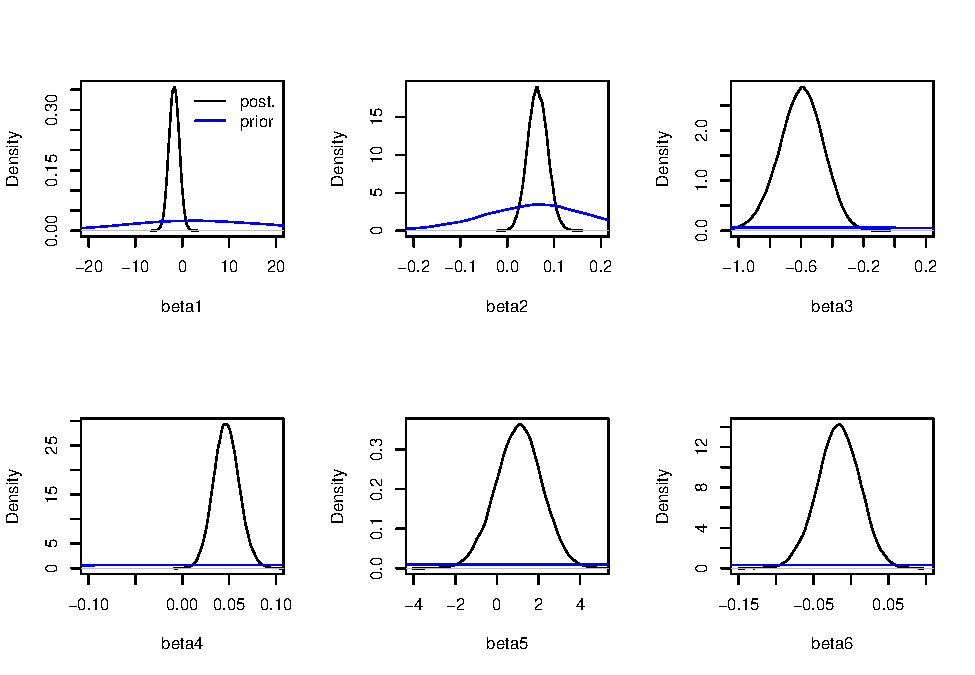
\includegraphics{Lab-3-Markdown_files/figure-latex/unnamed-chunk-5-1.pdf}

3a.

\begin{table}[h]

\begin{center}
\begin{threeparttable}

\caption{\label{tab:unnamed-chunk-6}Estimates and Standard Deviations of Coefficients in Prior Model and Posterior Models with n=100 and n=300.}

\begin{tabular}{rcccccc}
\toprule
Beta Coefficient & Prior mean & Prior SD & Mean|n=100 & SD|n=100 & Mean|n=300 & SD|n=300\\
\midrule
beta1 & 4.58 & 16.67 & -2.07 & 1.43 & -1.74 & 1.10\\
beta2 & 0.06 & 0.12 & 0.07 & 0.03 & 0.06 & 0.02\\
beta3 & -3.03 & 6.51 & -0.45 & 0.19 & -0.60 & 0.14\\
beta4 & 0.25 & 0.59 & 0.03 & 0.02 & 0.05 & 0.01\\
beta5 & 15.76 & 41.60 & -0.83 & 1.51 & 1.06 & 1.11\\
beta6 & -0.44 & 1.18 & 0.02 & 0.04 & -0.02 & 0.03\\
\bottomrule
\end{tabular}

\end{threeparttable}
\end{center}

\end{table}

\newpage

3b.

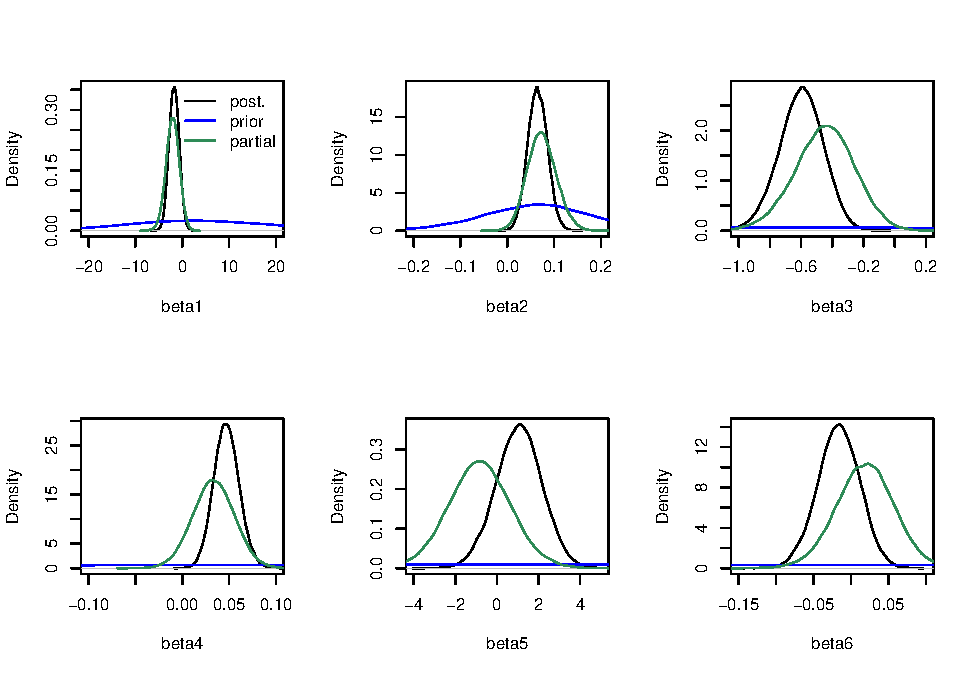
\includegraphics{Lab-3-Markdown_files/figure-latex/unnamed-chunk-7-1.pdf}

\begin{enumerate}
\def\labelenumi{\arabic{enumi}.}
\setcounter{enumi}{3}
\item
  The model tracks the parameters π1 to π6, what is the interpretation
  of these parameters once the data has been incorporated?\\
  The parameters \(\pi_{1:6}\) in the model represent the probability of
  death for the 6 hypothetical cases elicited from Dr.~Osler. Once the
  data has been incorporated, the updated values for \(\pi_i\) represent
  the posterior estimated mean probability of death for these six cases,
  with slightly larger variance.
\item
  Extra credit: you may (but don't need to) Turn in your answer to TODO
  step 3.\\
  An attempt was made! I added three lines to predict hypothetical
  observaitons by adding
  \texttt{futurepie1\ \textless{}-\ ilogit(betas{[}1{]}\ +\ betas{[}2{]}*2\ +\ betas{[}3{]}*7.55\ +\ betas{[}4{]}*25\ +\ betas{[}5{]}*0\ +\ betas{[}6{]}*0)}
  and so forth in three lines after defining the inverse logit
  regression's closed brackets. I managed to get Jags to run,
  incredibly.\\
  The table below shows the posterior estimates for the three cases,
  where the posterior probability (or do I say inverse log odds? I'm not
  used speaking about logistic regression) of death for case 1 = 1\%,
  case 2 = 4\%, and case 3 = 18\%.
\end{enumerate}

\begin{table}[h]

\begin{center}
\begin{threeparttable}

\caption{\label{tab:unnamed-chunk-9}Summary of Paramters for Hypothetical Observations}

\begin{tabular}{lccccc}
\toprule
Parameter & Mean & SD & 2.5 & 97.5 & p>0\\
\midrule
case1 & 0.01 & 0.00 & 0.00 & 0.02 & 1.00\\
case2 & 0.04 & 0.02 & 0.01 & 0.09 & 1.00\\
case3 & 0.18 & 0.16 & 0.01 & 0.60 & 1.00\\
\bottomrule
\end{tabular}

\end{threeparttable}
\end{center}

\end{table}

\end{document}
